\vspace*{\fill}
In this closing part, we conclude our work.
We do this by first giving a summary of our three main contributions \ref{cha:summary}: (i) The SimRa platform along with the mechanism for automatically deriving incidents, (ii) an approach for deriving road surface quality from smartphone-based \ac{imu} data and its integration into SimRa, and (iii) the derivation of a more realistic cyclist simulation for the traffic simulation software \ac{sumo}.
Lastly, in \Cref{cha:discussion_and_outlook}, we discuss the general constraints of our work and give an outlook on future work.
\vspace*{\fill}
\chapter{Summary}
\label{cha:summary}
Increasing the modal share of bicycle traffic comes with a plethora of benefits.
The reduction of greenhouse gas emissions has a positive impact both locally and globally.
The air, especially in urban areas, gets more clean and this comes with a higher quality of living and lower risk of medical problems.
The decrease in greenhouse gas emissions also slows down the global climate crisis, which is one of the main challenges of the 21st century.
Another benefit of an increase in bicycle traffic is, is that bicycle infrastructure needs less space than car infrastructure.
In many cities, a lack of space has lead to a housing crisis and less space for car infrastructure means more space for housing, which in turn can decrease the severity of the housing crisis.
These are just some benefits of increasing the modal share of bicycle traffic, which is why both government agencies and citizens want to boost cycling as a means to commute.
However, we identified these problems in \Cref{sec:problem} of \Cref{cha:introduction}:

\begin{itemize}
\item While there are statistics available regarding the incidence of accidents involving bicycles, there is a paucity of data concerning incidents that do not result in injury or death.
Such data is essential for understanding the locations and causes of incidents in bicycle traffic.
By identifying the locations and causes of incidents, city planners can implement infrastructure changes to enhance the safety and appeal of cycling.
Safety concerns are a primary deterrent for many individuals who are reluctant to cycle or who limit their cycling due to perceived risks.
Even without any changes to the infrastructure, cyclists can circumvent the dangerous spots or be more attentive while passing through them, if they know about them.
However, gathering this information the traditional way with surveys and studies is expensive and difficult to do right, so a possible solution needs to be easy and resource-saving to implement.
\item Similar to safety concerns, a lack of comfort is also detrimental to cycling.
Cycling comfort is heavily influenced by the quality of the cycling infrastructure, especially the surface quality thereof.
So, an efficient means of measuring the road surface quality of cycling infrastructure can help in the same manner as before, by helping city planners detect the most urgent spots to be improved and by informing cyclists, who in turn can adjust their cycling route.
\item Having the information about dangerous hotspots in bicycle traffic is not enough though to act on it.
Since changes to traffic infrastructure are expensive to undertake, these changes need to be planned thoroughly and for changes to be approved by the administration, they need to be sure that the changes will in fact improve the traffic situation as desired.
This is where traffic simulation software can be used.
The new infrastructure can be modeled and, with a realistic simulation, it can be compared to the current state.
A realistic cyclist simulation model is crucial for this since the insights won't be representative otherwise.
However, creating cyclist simulation models is complex, since it is not very easy to obtain the relevant data for that.
This raises the need for an approach using existing data to derive realistic cycling models from it.
\end{itemize}

To address these three problems, we presented one solution each:

\begin{itemize}
\item We created \textit{SimRa}, a platform for detecting dangerous hotspots in bicycle traffic.
SimRa uses a crowdsourcing approach, where users of a smartphone application record their cycling trips and after each trip give detailed information about incidents that happened during the ride.
They can then upload their ride file, which is a time series containing the GPS trace, as well as \ac{imu} data, together with the incidents if any happened during the ride.
Since remembering every incident and its specifics during a ride is a difficult task for the user, we implemented a feature which automatically detects incidents using a \ac{dl} model called \textit{CycleSense}.
\textit{CycleSense} can confidently propose exact locations along the cycling trip where an incident might have happened, which makes the reporting of the incidents easier for the users.
This, in turn, helps to record every incident that occurred during a ride without forgetting one and due to a better user experience also contributes to a higher user count and thus more representative data. 
With the SimRa dataset, city planners have an important information source where they need to focus their attention when working to improve bicycle safety in their area of responsibility.
On the other hand, citizens can use the data to increase pressure on the policymakers to act and to improve the situation for cyclists.
Additionally, they can inform themselves about the dangerous locations in bicycle traffic and avoid them.
\item We developed an approach for deriving the road surface quality from cycling trip data, that contains GPS and \ac{imu} data readings.
Notably, we designed our approach, so it can easily be integrated into any preexisting solution or dataset containing cycling trip data, fulfilling the requirements mentioned before.
We also have shown how we integrated this approach into \textit{SimRa} and created a visualization of the results.
The aforementioned information allows transportation departments to readily monitor the condition of their bicycle infrastructure and implement maintenance procedures in a more streamlined and effective manner.
Additionally, cyclists have access to more comprehensive information, which enables them to plan their cycling trips with greater precision.
Some cyclists may opt for a detour in order to enhance their cycling experience.
\item We improved the cyclist simulation model of \ac{sumo}.
We did this by first examining the lateral movement and intersection behavior of cyclists with the SimRa dataset and comparing it to the existing cyclist simulation model of \ac{sumo}. 
Our analysis showed that \ac{sumo}'s cyclist model is very unrealistic, which is hardly surprising, considering the fact, that \ac{sumo} simulates cyclists either as fast pedestrians or slow cars.
We then inferred the three different cyclist types \textit{slow}, \textit{medium}, and \textit{fast} by splitting  the rides of the SimRa dataset into three parts by their speed.
For each subset, we calculated the acceleration, deceleration, and maximum velocity distributions, as well as their left-turn behavior at intersections.
We implemented our findings as \ac{sumo} plugins so that users can use them in their simulations.
With this, e.g., city planners can use three different cyclist types, which are all more realistic than the default cyclist model of \ac{sumo}.
In doing so, they can better plan the way they want to change the bicycle infrastructure. 
\end{itemize}

This thesis consists of three parts. \Cref{part:foundations}, Foundations, begins with an introduction to the topic, the motivation of this thesis, the problem statements, as well as the structure.

\Cref{part:contributions}, Improving Safety in Bicycle Traffic, contains all of our main contributions.
In \Cref{cha:cyclesense} we introduced \textit{SimRa}, a platform for gathering cycling trip and incident data, as well as our approach to automatically detect incidents from \ac{imu} data from cycling trips, called \textit{CycleSense}.
We then presented an approach to derive road surface quality from bicycle trip data in \Cref{cha:cyclequality}.
There, we also showed how to integrate our approach into an existing cycling trip recording app by integrating the approach into \textit{SimRa} and how the results can be visualized.
In \Cref{cha:sumo}, which is the last chapter of \Cref{part:contributions}, we showed how we extract parameters for acceleration, deceleration, and velocity of cyclists, as well as their left-turn behavior at intersections.
We also showed, how we implement our findings as a plugin for \ac{sumo}.
\Cref{cha:cyclesense,cha:cyclequality,cha:sumo} are structured very similarly.
They start with a brief introduction, continue with background information, a description, an evaluation, a discussion of the approach, and end with an overview of alternative approaches and a conclusion.

In \Cref{part:conclusions}, Conclusions, we concluded this thesis with a summary in \Cref{cha:summary} a discussion of our work, and an outlook for future work in \Cref{sec:outlook}.
\chapter{Discussion and Outlook}
\label{cha:discussion_and_outlook}
In this chapter, we discuss the limitations of our approach and give an outlook for future work.
While we discuss the limitations of each contribution in their respective chapters in \Cref{part:contributions}, there are some limitations, that they share, which we collect here.
This chapter contains partially adapted material published in \cite{karakaya2020simra,karakaya2022cyclesense,karakaya2022realistic,karakaya2023achieving,karakaya2023crowdsensing}.

\section{Limitations of Crowdsourced Data}
\label{sec:limitations_of_crowdsourced_data}
Crowdsourced data are generally noisy which could contribute to a reduced model performance.
They also contain several biases, e.g., Selection Bias, Device Positioning Bias, Extreme Aversion Bias, or Confirmation Bias~\cite{basiri2019crowdsourced, chakraborty2017makes, kahneman1991anomalies}.
In this context, the heterogeneity across devices and platforms is likely another factor of influence.
As already described, the application that is used by contributors to record their rides is available on two platforms. 
Those platforms are supported by a wide range of different devices and models with different hardware inside. 
Phone manufacturers use different \ac{gps}, gyroscope, and accelerometer sensors that can vary immensely in sensitivity and overall behavior.
Stisen et al.~\cite{stisen2015smart} have shown that there is major heterogeneity when it comes to the accuracy of sensor readings. 
While the main focus of that study was on accelerometer data, Kuhlmann et al.~\cite{kuhlmann2021smartphone} have shown that orientation sensor data is also affected by this variability.
\subsection*{Implications for Gathering Cycling Trip Data and Detecting Incidents}
This is in contrast to the \ac{har} tasks, we compared our task to in \Cref{cha:cyclesense}.
The \ac{har} data set~\cite{anguita2013public} was generated under laboratory conditions that always used the same smartphone type body mounted to the exact same position on selected study participants.
This significantly simplifies the classification task.
Another factor that contributes to the issue of noisy crowdsourcing data in the SimRa data set is the fact that some users misinterpret the purpose of the SimRa app.
Instead of labeling incidents, they report, e.g., dangerous areas or annoying traffic lights.
These can of course not be captured by the sensors used.
Many such ``incidents'' can be identified through the comment column of the data set.
It should also be noted that the SimRa data set was not recorded and labeled with the goal of developing ML models -- the goal was to record data that will be analyzed and processed by humans.

\subsection*{Implications for Deriving Road Surface Quality from Cycling Trip Data}
Heterogeneous \ac{imu} data poses also a challenge when deriving road surface quality, as we did in \Cref{cha:cyclequality}.
This stems from the fact that different smartphone models have different GPS modules and motion sensors, which leads to the problem that a road can be very smooth according to one smartphone and very rough according to another.
This problem is further aggravated by the wide range of different bicycle types, e.g., racing bicycles or mountain bikes, which in turn also heavily influence the vibrations the smartphone can sense.
To solve these problems, we rely on the \textit{law of large numbers} and compare how a section's surface quality was relative to the ride. 

\section{Limitations of the Preprocessing in SimRa}
It is important to note, that SimRa was developed for identifying incident hotspots in bicycle traffic.
For that, a relatively low accelerometer sampling rate of 50 Hz is used before further reducing the level of detail by calculating the moving average with a window size of 30 and then taking every fifth value.

\subsection*{Implications for Gathering Cycling Trip Data and Detecting Incidents}
Recording rates of sensor readings deviate among devices and operating systems and impair model predictions~\cite{stisen2015smart}, this may also affect the performance of \textit{CycleSense}:
As illustrated in Figure~\ref{fig:emp-measurements}, the recording rates differ significantly in older and newer Android rides as well as in iOS rides.
While the iOS rides' median ($\approx$ 300 ms) is similar to the one of newer Android rides, the \ac{iqr} is much greater and spans approximately 150 ms.
This circumstance could indicate that the relatively weak model performance on this data set can partly be explained by that factor. 
Furthermore, the gyroscope data is recorded with a higher frequency in newer Android rides than in older Android or iOS rides.
This factor could also contribute to the different model evaluation results. 
The achieved \ac{auc} \ac{roc} for uncleaned newer Android data was 0.870, while it was 0.823 for the older Android data.

\begin{figure}[t]
	\centering
	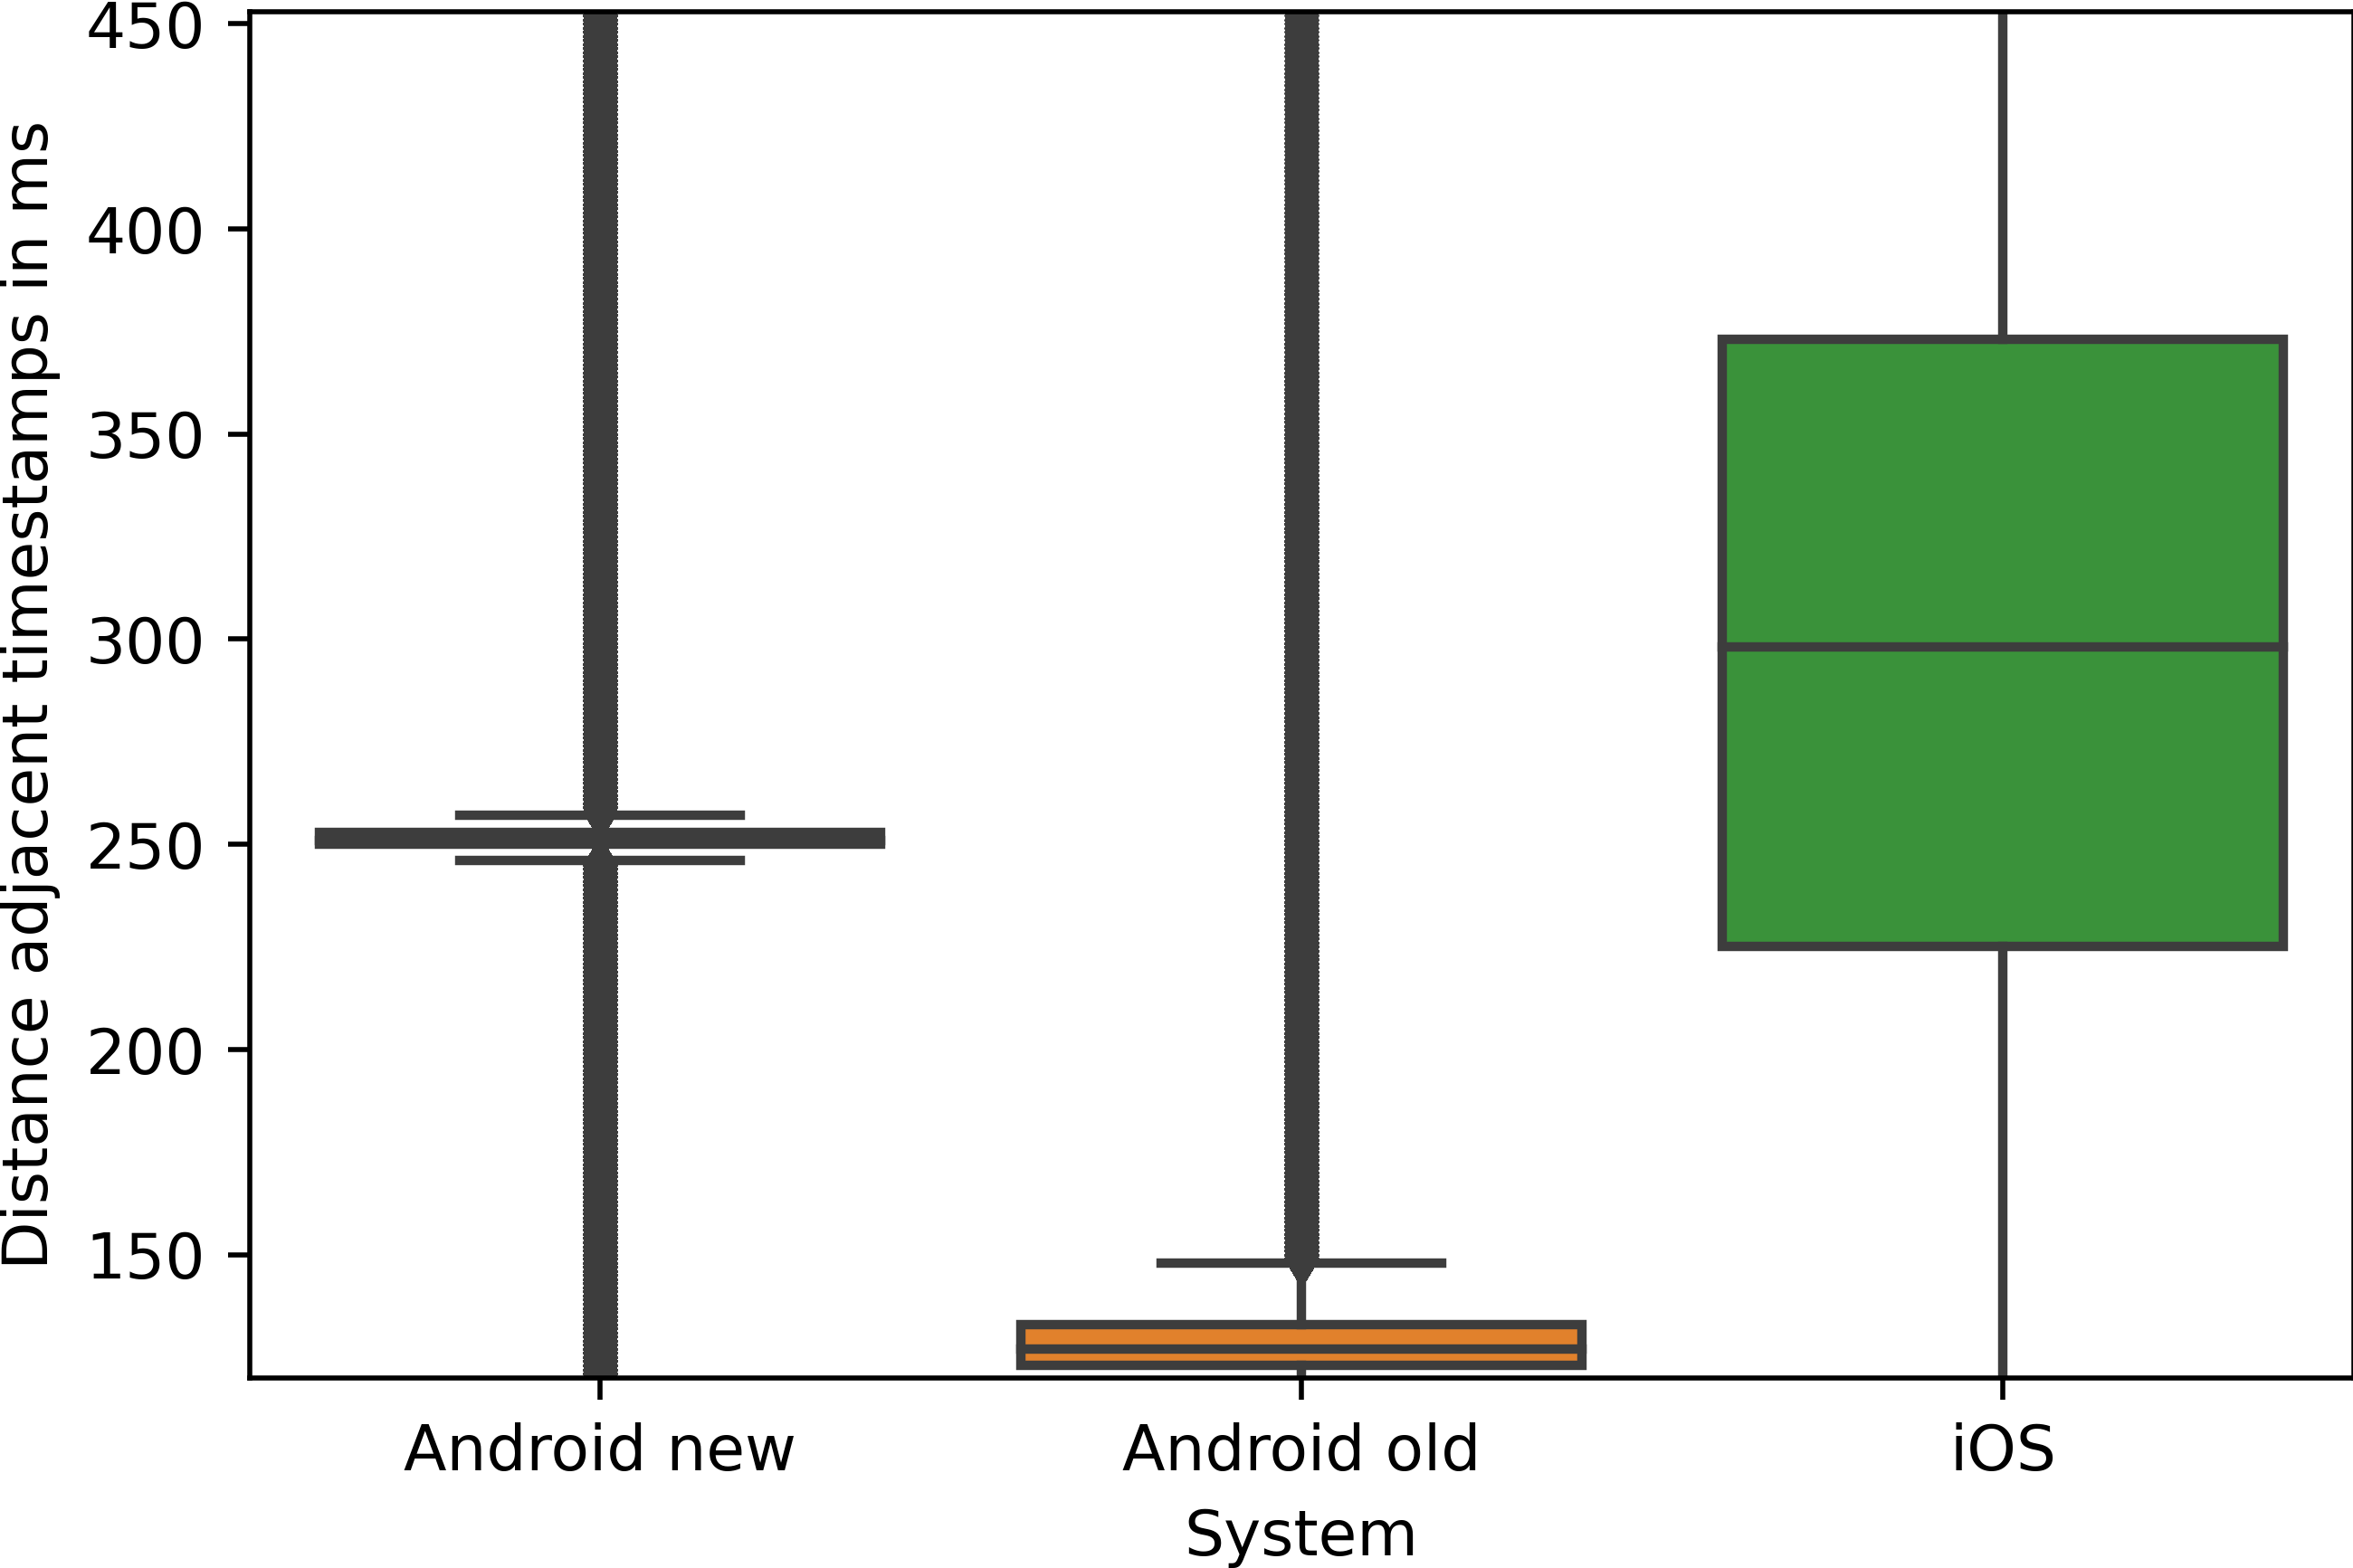
\includegraphics[width=0.45\textwidth]{fig/empirical_measurements.png}
	\caption{Box plot showing the empirical measurement times observed in the SimRa data set for rides recorded with different versions of the SimRa app.}
	\label{fig:emp-measurements}
\end{figure}

Aside from that, the moving average that is used in the SimRa app to condense the data and comply with users' upload volume constraints~\cite{karakaya2020simra} reduces the amplitude and shifts the exact point in time of incidents and other events.
This has the effect that incidents and non-incidents are hard to distinguish as illustrated in Figure~\ref{fig:heavy-vs-normal-braking}.
Both these factors could hurt the model's ability to classify incidents correctly based on the data.
It is important to acknowledge that this issue becomes less severe when the sampling frequency is higher, as it is the case for the older Android data.

\begin{figure}[t]
	\centering
	\begin{subfigure}[b]{0.475\textwidth}
		\centering
		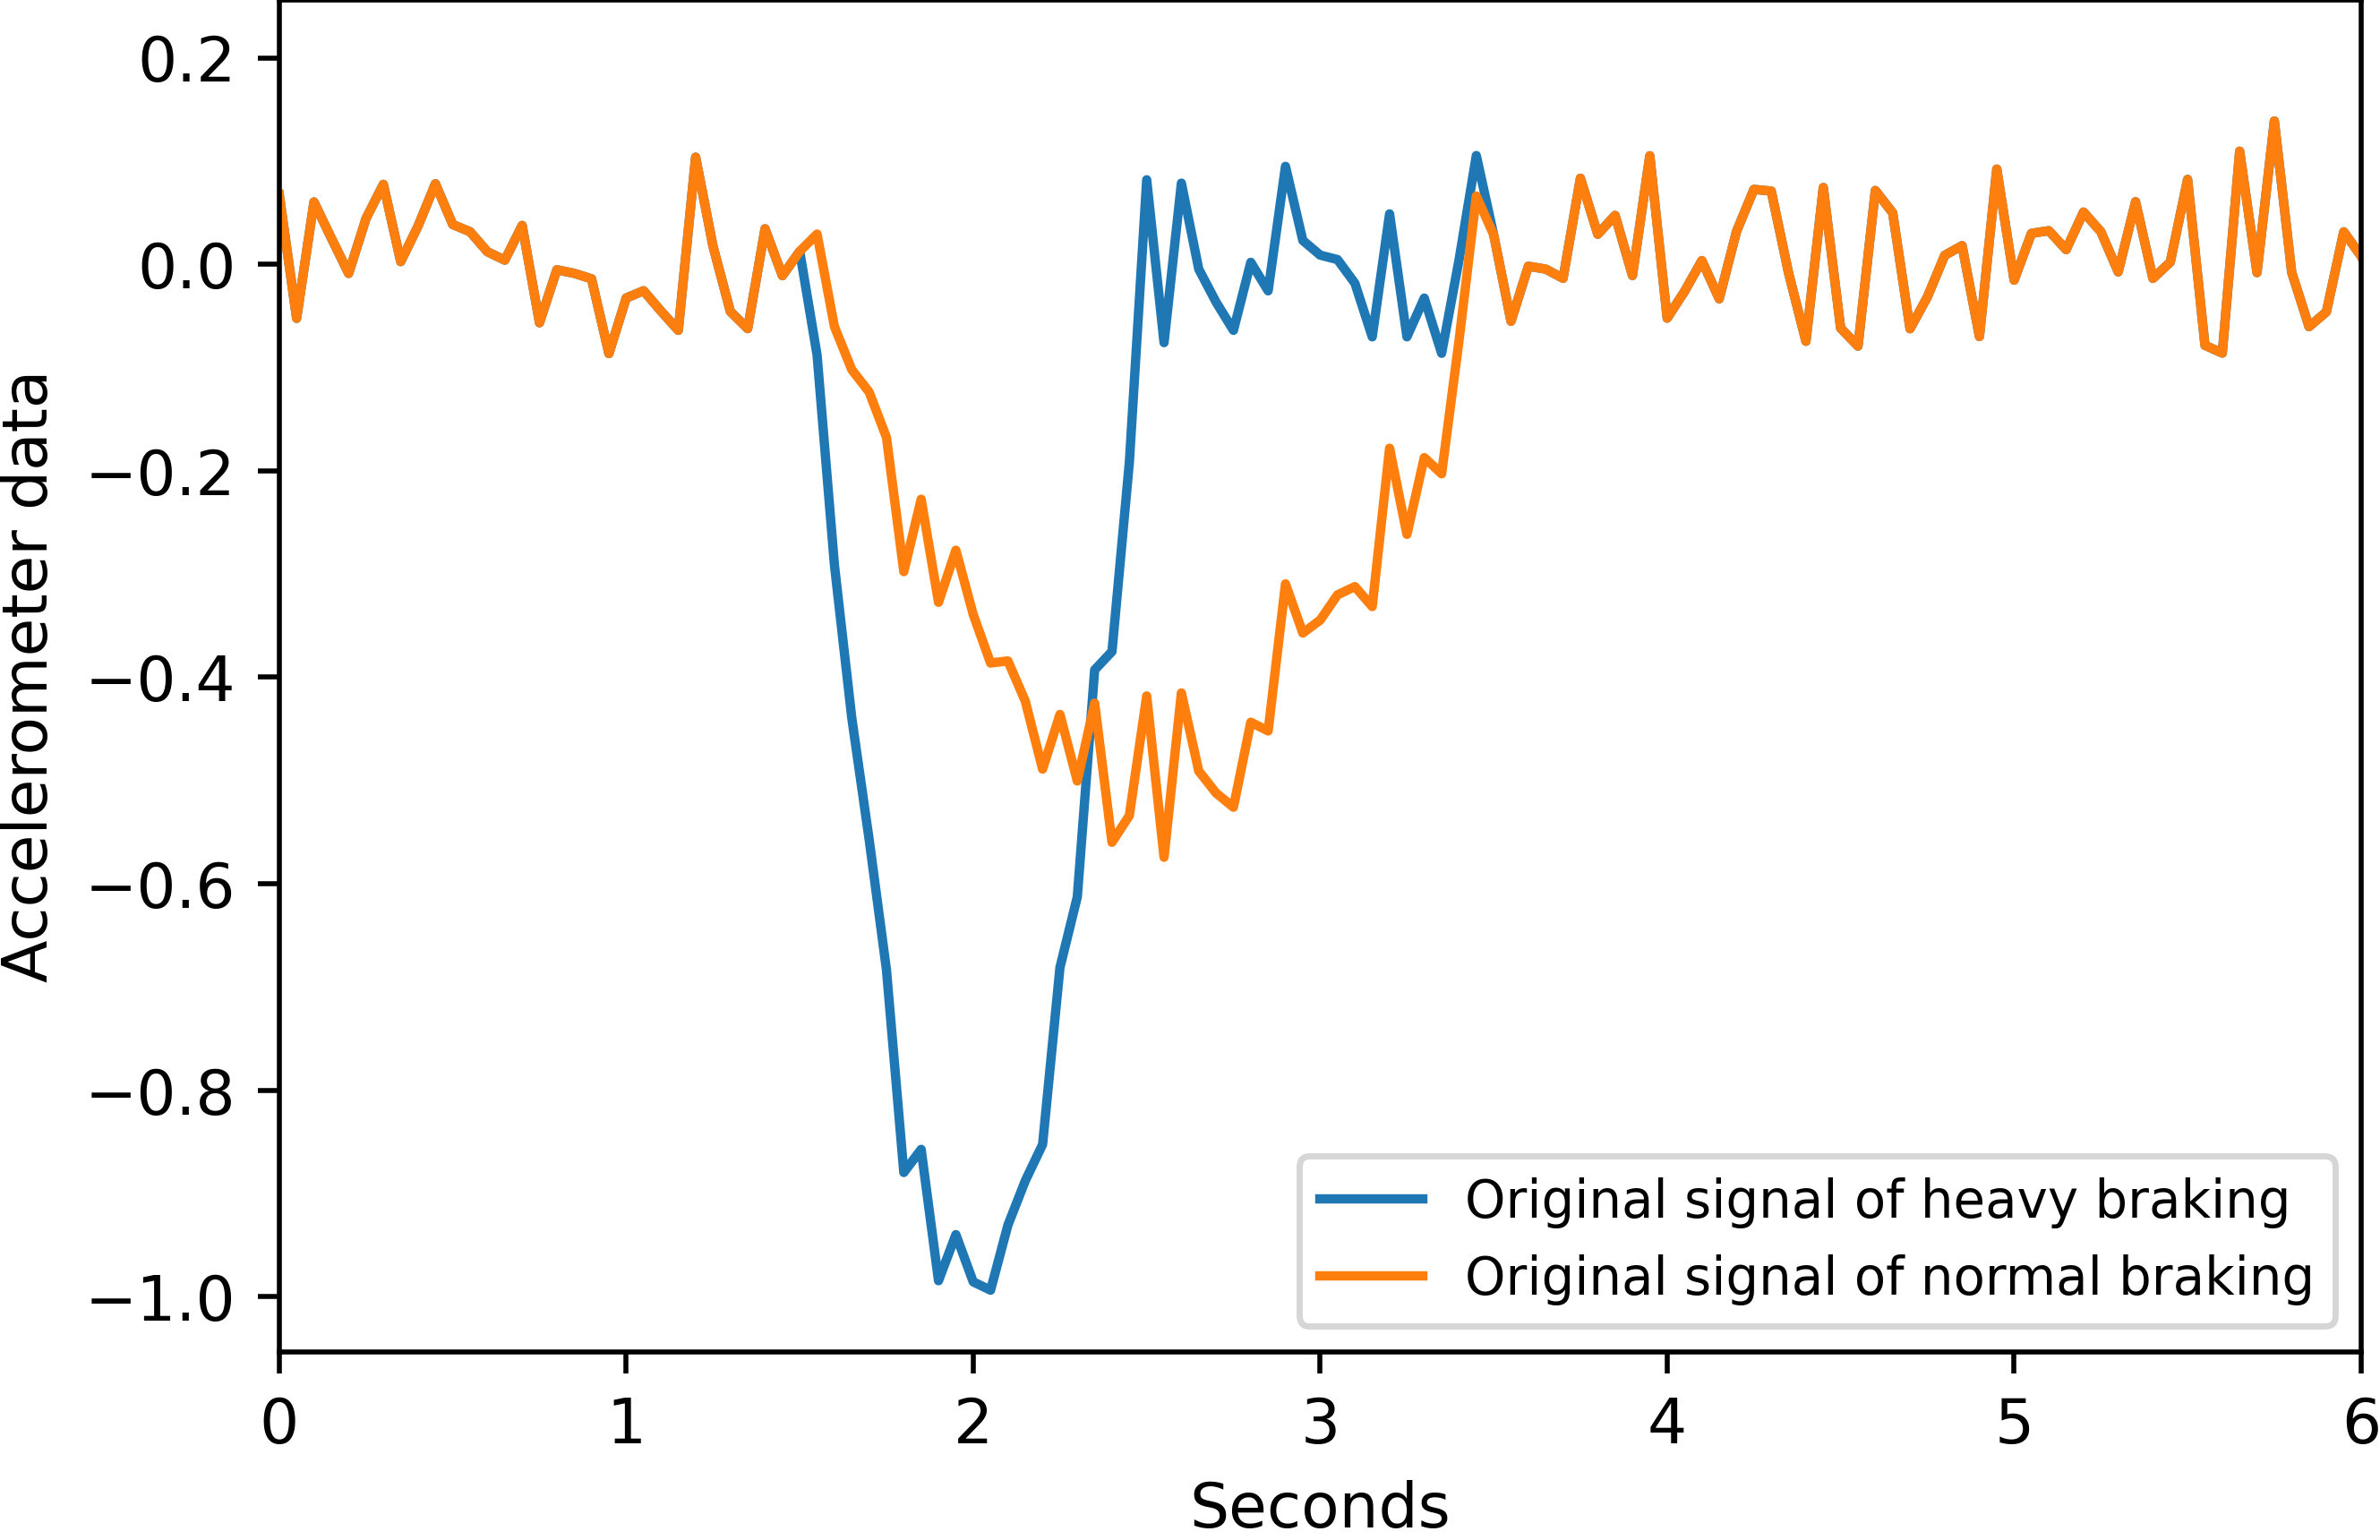
\includegraphics[width=\textwidth]{fig/heavy_vs_normal_braking}
		%\caption{\small Scaled accelerometer data over time of the original signal of an artificially modeled incident with heavy braking vs.\ an artificially modeled moderate braking event.}
	\end{subfigure}
	\hfill
	\begin{subfigure}[b]{0.475\textwidth}
		\centering
		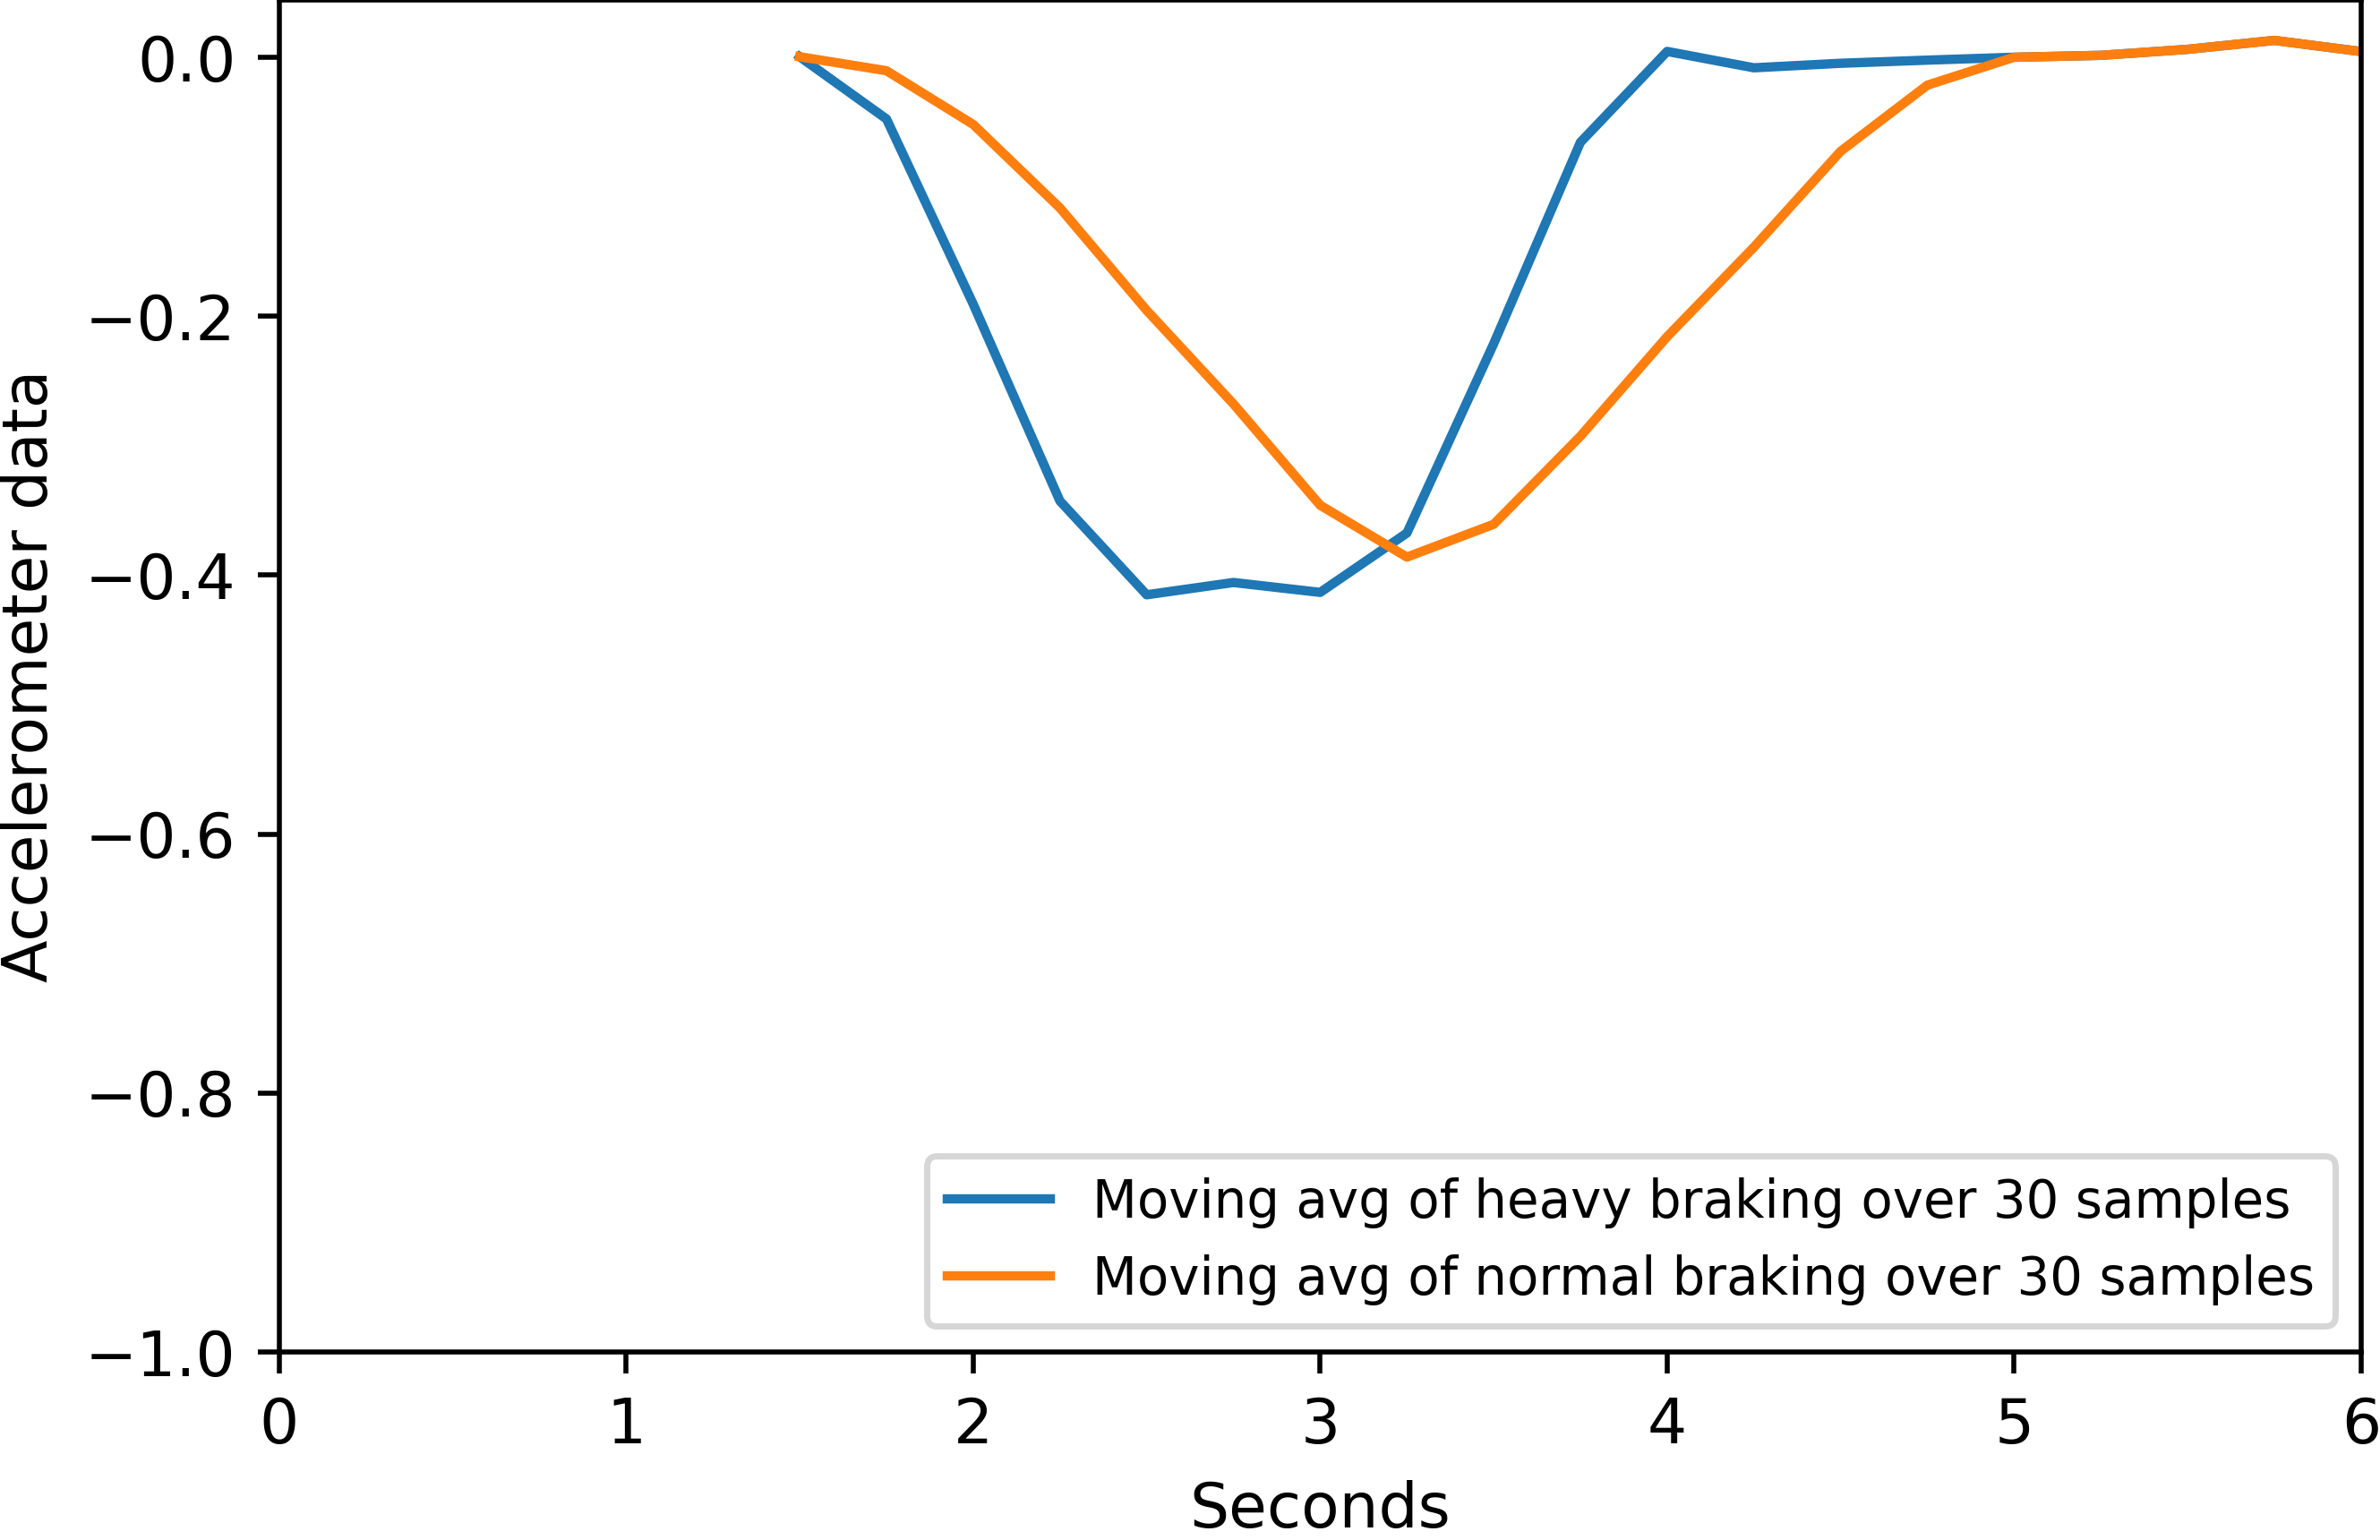
\includegraphics[width=\textwidth]{fig/mvn_avg_heavy_vs_normal_braking.png}
		%\caption{\small Moving average applied on the scaled accelerometer data of the original signal of an artificially modeled incident with heavy braking vs.\ an artificially modeled moderate braking event.}
	\end{subfigure}	
	\caption{Visualization of the sensor data of a simulated heavy braking incident vs.\ a moderate braking event before and after the moving average has been applied.}
	\label{fig:heavy-vs-normal-braking}
\end{figure}

\subsection*{Implications for Gathering Cycling Trip Data and Detecting Incidents}
A higher resolution of data points would allow us to develop a more sophisticated measurement approach.
This would, however, further increase the disk space, memory, battery, and bandwidth usage of the SimRa app, and as we have shown in \Cref{sec:evaluation_cyclequality}, the surface quality we derive is sufficiently precise for our intended use cases.

\section{Outlook}
\label{sec:outlook}
A promising direction for future work is to explore the relationship between incidents and traffic infrastructure.
Since the \textit{SimRa} dataset contains incidents with their location and incident type, it might be possible to identify which conditions dangerous spots in traffic have in common.
E.g., it seems apparent that a narrow street without a protected bicycle lane would have a high risk for close passes.
However, such an analysis could reveal far more subtle connections between a certain traffic infrastructure characteristic and an incident type.

Similarly, climate and weather conditions can have an impact on the frequency and type of incidents, which also poses a promising topic.
Since the \textit{SimRa} dataset contains timestamps of the rides and incidents, the weather information can be considered to see if there are any correlations.
E.g., stormy weather, which impacts the perception of car drivers, could lead them to not see cyclists and thus make a right-turn, cutting the cyclists behind them, that wanted to cycle straight forward.

While we developed and provide visualizations\footnote{https://simra-project.github.io/dashboard/} showing the results of the \textit{SimRa} project, further tools can be developed to analyze the dataset in an intuitive manner.
In fact, the cities of Walldorf and Wiesloch, as well as the municipalities Zeuthen, Eichwalde, and Schulzendorf approached us with a request to develop tools with advanced analysis features for the \textit{SimRa} dataset.
This also shows that the \textit{SimRa} project is considered and used by administration bodies to improve the state of their bicycle traffic.
 